
\begin{figure}[htbp]
    \centering

    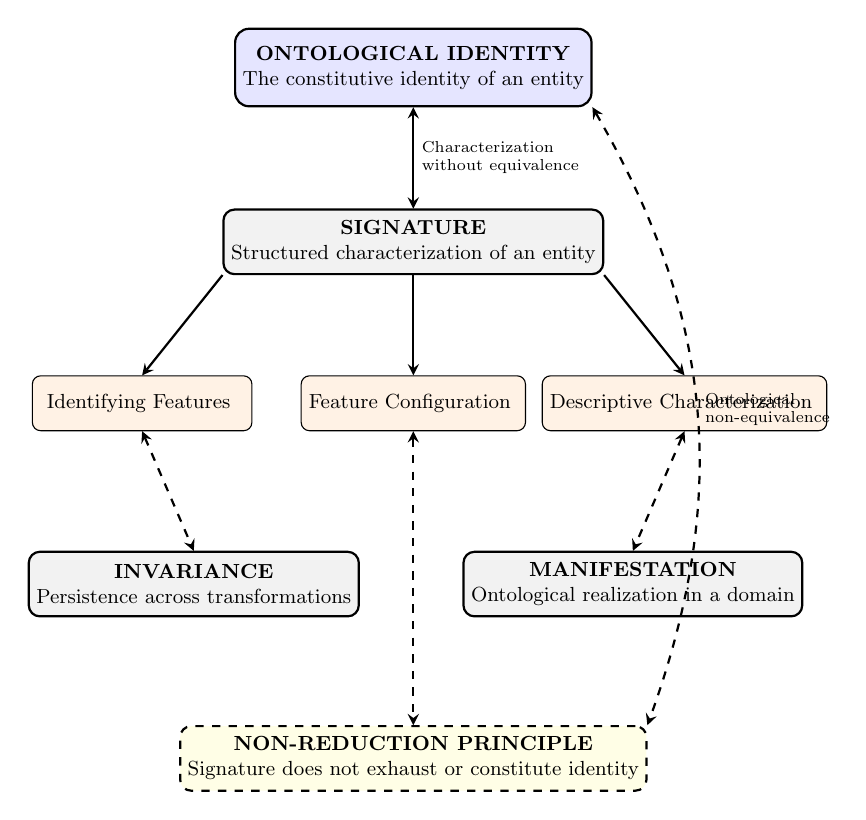
\begin{tikzpicture}[
        scale=0.82,
        transform shape,
        every node/.style={font=\small},
        core/.style={
            rectangle,
            rounded corners=5pt,
            draw=black,
            thick,
            minimum width=5.0cm,
            minimum height=1.2cm,
            align=center,
            fill=blue!10
        },
        concept/.style={
            rectangle,
            rounded corners=4pt,
            draw=black,
            thick,
            minimum width=4.3cm,
            minimum height=1.0cm,
            align=center,
            fill=gray!10
        },
        feature/.style={
            rectangle,
            rounded corners=3pt,
            draw=black,
            minimum width=3.4cm,
            minimum height=0.85cm,
            align=center,
            fill=orange!10
        },
        limit/.style={
            rectangle,
            rounded corners=4pt,
            draw=black,
            dashed,
            thick,
            minimum width=4.7cm,
            minimum height=1.0cm,
            align=center,
            fill=yellow!10
        },
        relation/.style={
            <->,
            thick,
            >=stealth
        },
        expression/.style={
            ->,
            thick,
            >=stealth
        },
        nonreduction/.style={
            dashed,
            thick,
            <->,
            >=stealth
        }
    ]

    % Ontological identity
    \node[core] (identity) at (0,0) {
        \textbf{ONTOLOGICAL IDENTITY}\\
        The constitutive identity of an entity
    };

    % Signature as structured characterization
    \node[concept] (signature) at (0,-2.7) {
        \textbf{SIGNATURE}\\
        Structured characterization of an entity
    };

    % Components of signature
    \node[feature] (features) at (-4.2,-5.2) {
        Identifying Features
    };

    \node[feature] (configuration) at (0,-5.2) {
        Feature Configuration
    };

    \node[feature] (description) at (4.2,-5.2) {
        Descriptive Characterization
    };

    % Related but non-equivalent dimensions
    \node[concept] (invariance) at (-3.4,-8.0) {
        \textbf{INVARIANCE}\\
        Persistence across transformations
    };

    \node[concept] (manifestation) at (3.4,-8.0) {
        \textbf{MANIFESTATION}\\
        Ontological realization in a domain
    };

    % Principle of non-reduction
    \node[limit] (limit) at (0,-10.7) {
        \textbf{NON-REDUCTION PRINCIPLE}\\
        Signature does not exhaust or constitute identity
    };

    % Identity and signature: characterization without equivalence
    \draw[relation]
        (identity.south) --
        node[right, align=left, font=\scriptsize] {
            Characterization\\
            without equivalence
        }
        (signature.north);

    % Signature and its descriptive components
    \draw[expression] (signature.south west) -- (features.north);
    \draw[expression] (signature.south) -- (configuration.north);
    \draw[expression] (signature.south east) -- (description.north);

    % Relations to invariance and manifestation
    \draw[nonreduction] (features.south) -- (invariance.north);
    \draw[nonreduction] (description.south) -- (manifestation.north);

    % Configuration does not constitute identity
    \draw[nonreduction] (configuration.south) -- (limit.north);

    % Explicit non-equivalence between identity and signature-based description
    \draw[nonreduction]
        (identity.south east)
        to[bend left=25]
        node[right, align=left, font=\scriptsize] {
            Ontological\\
            non-equivalence
        }
        (limit.north east);

    \end{tikzpicture}

    \caption{The Ontological Distinction Between Identity and Signature: Structured Characterization, Related Dimensions, and the Principle of Non-Reduction}
    \label{fig:identity-and-signature}
\end{figure}
